\chap{Timer Interrupt and LED Scanning}

\section{Introduction}
Timers are one of the most important features in modern micro-controllers. They allow us to measure how long something takes to execute, create non-blocking code, precisely control pin timing, and even run operating systems.\\

The STM32 line of micro-controllers from ST-Microelectronics are no exception: each controller offers a full suite of timers for us to use. In this manual, how to configure a timer using STM32CubeIDE is presented how to use them to flash an LED. Finally, students are proposed to finalize 10 exercises using timer interrupt for applications based LED Scanning.

\newpage
\section{Exercise and Report}
\subsection{Exercise 1}
The first exercise show how to interface for multiple seven segment LEDs to STM32F103C6 micro-controller (MCU). Seven segment displays are common anode type, meaning that the anode of all LEDs are tied together as a single terminal and cathodes are left alone as individual pins. \\

In order to save the resource of the MCU, individual cathode pins from all the seven segment LEDs are connected together, and connect to 7 pins of the MCU. These pins are popular known as the \textbf{signal pins}. Meanwhile, the anode pin of each seven segment LEDs are controlled under a power enabling circuit, for instance, an PNP transistor. At a given time, only one seven segment LED is turned on. However, if the delay is small enough, it seems that all LEDs are enabling. \\

Implement the circuit simulation in Proteus with two 7-SEGMENT LEDs as following:

\begin{figure}[!htp]
    \centering
    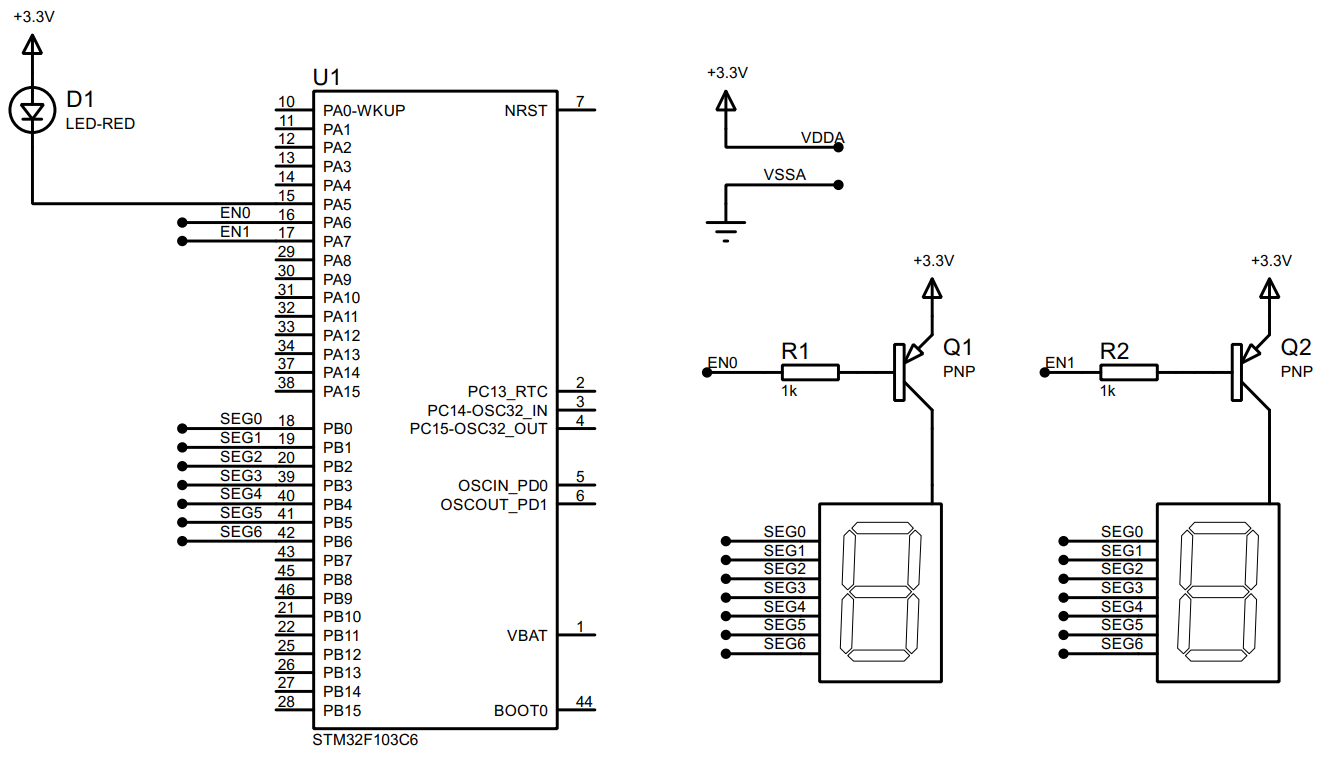
\includegraphics[width=5.5in]{source/picture/bai_2/lab2_ex1a.PNG}
    \caption{\textit{Simulation schematic in Proteus}}
    \label{bai2_pic1a}
\end{figure}
Components used in the schematic are listed bellow:
\begin{itemize}
    \item 7SEG-COM-ANODE (connected from PB0 to PB6)
    \item LED-RED
    \item PNP
    \item RES
    \item STM32F103C6
\end{itemize}


Students are proposed to use the function \textbf{display7SEG(int num)} in the Lab 1 in this exercise. Implement the source code in the interrupt callback function to display number \textbf{"1"} on the first seven segment and number \textbf{"2"} for second one. The switching time between 2 LEDs is half of second. \\

\textbf{Report 1: } Capture your schematic from Proteus and show in the report.\\

\textbf{Report 2: } Present your source code in the \textbf{HAL\_TIM\_PeriodElapsedCallback} function.\\

\textbf{Short question: } What is the frequency of the scanning process?\\

\subsection{Exercise 2}
Extend to 4 seven segment LEDs and two LEDs (connected to PA4, labeled as \textbf{DOT}) in the middle as following:

\begin{figure}[!htp]
    \centering
    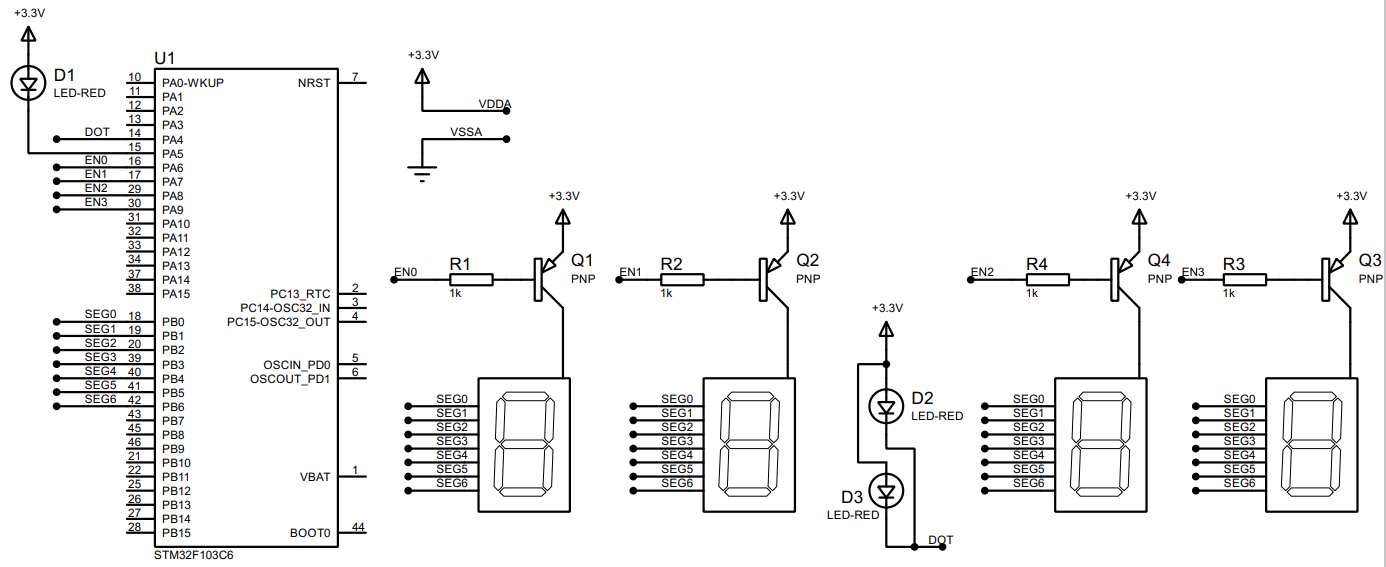
\includegraphics[width=5.5in]{source/picture/bai_2/lab2_ex2a.PNG}
    \caption{\textit{Simulation schematic in Proteus}}
    \label{bai2_pic1a}
\end{figure}

Blink the two LEDs every second. Meanwhile, number 3 is displayed on the third seven segment and number 0 is displayed on the last one (to present 12 hour and a half). The switching time for each seven segment LED is also a half of second (500ms). \textbf{Implement your code in the timer interrupt function.}\\

\textbf{Report 1: } Capture your schematic from Proteus and show in the report.\\

\textbf{Report 2: } Present your source code in the \textbf{HAL\_TIM\_PeriodElapsedCallback} function.\\

\textbf{Short question: } What is the frequency of the scanning process?\\

\subsection{Exercise 3}
Implement a function named \textbf{update7SEG(int index)}. An array of 4 integer numbers are declared in this case. The code skeleton in this exercise is presented as following:
\newpage
\begin{lstlisting}[caption=An example for your source code]
const int MAX_LED = 4;
int index_led = 0;
int led_buffer[4] = {1, 2, 3, 4};
void update7SEG(int index){
    switch (index){
        case 0:
            //Display the first 7SEG with led_buffer[0]
            break;
        case 1:
            //Display the second 7SEG with led_buffer[1]
            break;
        case 2:
            //Display the third 7SEG with led_buffer[2]
            break;
        case 3:
            //Display the forth 7SEG with led_buffer[3]
            break;
        default:
            break;
    }
}
\end{lstlisting}

This function should be invoked in the timer interrupt, e.g update7SEG(index\_led++). The variable \textbf{index\_led} is updated to stay in a valid range, which is from 0 to 3. \\

\textbf{Report 1: } Present the source code of the update7SEG function. \\

\textbf{Report 2: } Present the source code in the HAL\_TIM\_PeriodElapsedCallback.\\

Students are proposed to change the values in the \textbf{led\_buffer} array for unit test this function, which is used afterward.

\subsection{Exercise 4}
Change the period of invoking update7SEG function in order to set the frequency of 4 seven segment LEDs to 1Hz. The DOT is still blinking every second


\textbf{Report 1: } Present the source code in the \textbf{HAL\_TIM\_PeriodElapsedCallback}. \\